\documentclass[10pt]{article}
\usepackage{tikz}
\usetikzlibrary{shapes.misc}
\usepackage[margin=0cm]{geometry}
\pagestyle{empty}
\tikzstyle{every node}=[cross out, draw, red]

\begin{document}

\vspace*{\fill}
\begin{center}
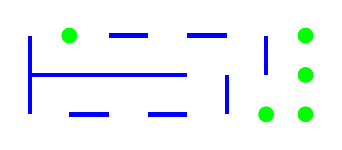
\begin{tikzpicture}[x=0.5cm, y=-0.5cm, ultra thick, blue]
% Walls
    \draw (2,0) -- (3,0);
    \draw (4,0) -- (5,0);
    \draw (0,1) -- (4,1);
    \draw (1,2) -- (2,2);
    \draw (3,2) -- (4,2);
    \draw (0,0) -- (0,2);
    \draw (5,1) -- (5,2);
    \draw (6,0) -- (6,1);
% Pillars
    \fill[green] (1,0) circle(0.2);
    \fill[green] (7,0) circle(0.2);
    \fill[green] (7,1) circle(0.2);
    \fill[green] (6,2) circle(0.2);
    \fill[green] (7,2) circle(0.2);
% Inner points in accessible cul-de-sacs
% Entry-exit paths without intersections
\end{tikzpicture}
\end{center}
\vspace*{\fill}

\end{document}
